%
% One column figure
%-----------------------------------------------------------
   \begin{figure}
   \centering
\tikzstyle{smallfig}=[scale=0.25]
   %
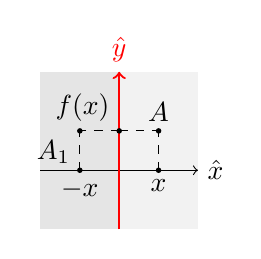
\begin{tikzpicture}[style=smallfig]
\fill [lightgray!20] (0, -3) rectangle (4, 5);
\fill [lightgray!40] (-4, -3) rectangle (0, 5);

\draw[thin,->] (-4,0) -- (4,0) node[right] {$\hat{x}$};
\draw[thick,->,red] (0,-3) -- (0,5) node[above] {$\hat{y}$};

\fill (2,2) circle (4pt) node[above] {$A$};
\draw[dashed,thin,-] (0,2.0) -- (2,2.0);
\fill (0,2) circle (4pt) node[above left] {$f(x)$};
\draw[dashed,thin,-] (2,0) node[below] {$x$} -- (2,2);
\fill (2,0) circle (4pt);
\fill (-2,2) circle (4pt) node[below left] {$A_1$};
\draw[dashed,thin,-] (0,2.0) -- (-2,2.0);
\draw[dashed,thin,-] (-2,0) node[below] {$-x$} -- (-2,2);
\fill (-2,0) circle (4pt);
\end{tikzpicture}
\quad
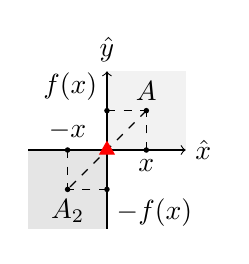
\begin{tikzpicture}[style=smallfig]
\fill [lightgray!20] (0, 0) rectangle (4, 4);
\fill [lightgray!40] (-4, -4) rectangle (0, 0);

\draw[thin,->] (-4,0) -- (4,0) node[right] {$\hat{x}$};
\draw[thin,->] (0,-4) -- (0,4) node[above] {$\hat{y}$};

\fill (2,2) circle (4pt) node[above] {$A$};
\draw[dashed,thin,-] (0,2.0) -- (2,2.0);
\fill (0,2) circle (4pt) node[above left] {$f(x)$};
\draw[dashed,thin,-] (2,0) node[below] {$x$} -- (2,2);
\fill (2,0) circle (4pt);
\fill (-2,-2) circle (4pt) node[below] {$A_2$};
\draw[dashed,thin,-] (0,-2) node[below right] {$-f(x)$} -- (-2,-2);
\draw[dashed,thin,-] (-2,0) node[above] {$-x$} -- (-2,-2);
\fill (0,-2) circle (4pt);
\draw[dashed,thin,-] (2,2) -- (-2,-2);
\fill (-2,0) circle (4pt);

\node[mark size=3pt,color=red] at (0,0) {\pgfuseplotmark{triangle*}};
\end{tikzpicture}
\quad
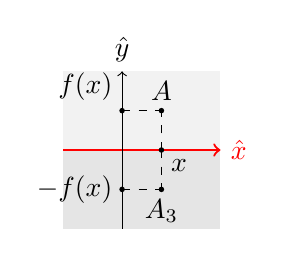
\begin{tikzpicture}[style=smallfig]
\fill [lightgray!20] (-3, 0) rectangle (5, 4);
\fill [lightgray!40] (-3, -4) rectangle (5, 0);

\draw[thick,->,red] (-3,0) -- (5,0) node[right] {$\hat{x}$};
\draw[thin,->] (0,-4) -- (0,4) node[above] {$\hat{y}$};

\fill (2,2) circle (4pt) node[above] {$A$};
\draw[dashed,thin,-] (0,2.0) -- (2,2.0);
\fill (0,2) circle (4pt) node[above left] {$f(x)$};
\draw[dashed,thin,-] (2,0) node[below right] {$x$} -- (2,2);
\fill (2,0) circle (4pt);
\fill (2,-2) circle (4pt) node[below] {$A_3$};
\draw[dashed,thin,-] (2,0) -- (2,-2);
\draw[dashed,thin,-] (0,-2) node[left] {$-f(x)$} -- (2,-2);
\fill (0,-2) circle (4pt);
\end{tikzpicture}
   %
   \caption{The three symmetrical copies of $f$. From left to
    right: vertical, center and horizontal symmetries.}
   \label{fig:symms}
   \end{figure}
%-----------------------------------------------------------
%